\chapter{TruMan}
\label{chap:truman}

This work shows that it is possible to adapt a trust management scheme originally designed for static networks to a dynamic environment, such as a VANET.
In order to make this possible, it is necessary to identify features in VANETs that show that nodes can share a long-term relationship, as is the case for social networks.
%The arguments for such features are presented in \autoref{section:socialvanets}, while the movement model that enables the simulation of the features is explained in \autoref{section:workingday}.
Through these long-term relationships, it then becomes feasible for nodes to store trust data and share it with other nodes.
By combining a node's own opinions about familiar nodes and trust information received from its neighbors, it is possible to create a model of the surrounding network.
This model includes a trust graph, showing the trust relationships between pair of nodes, which can then be used as in conjunction with other algorithms in order to classify nodes as correct or malicious.

%The previous chapters show why vehicular networks require distinguished trust models compared to social networks and traditional MANETs.
%In this chapter, it is proposed that certain aspects from social networks can be found in vehicular networks and, through those aspects, it is possible to adapt a trust model designed for traditional complex networks to a vehicular environment.
%These social properties allow for long-term trust relationships to be established amongst nodes of a network and, therefore, previously existing trust models can be adapted to the vehicular environment.

In this chapter, the reasoning behind TruMan and details of how it works are presented.
First, it is shown how vehicles can form long-term relationships and trust one another in a similar way to social networks.
Then, two algorithms are introduced: Tarjan's strongly connected components algorithm \citep{tarjan1972depth} and an efficient algorithm for graph coloring \citep{mittal2011graph}.
Next, the Malicious Node Identification Algorithm (MaNI) \citep{vernize2013dissertation} is explained, for it is the work that suggests the usage of strongly connected components and graph coloring for malicious node detection.
Finally, TruMan itself is explained, showing how it combines features from existing algorithms and adapts them to a dynamic environment, enabled by the social properties found in vehicular networks.
%Then, the Working Day Movement Model is introduced, along with the reasons why it is best fitted for this work.
%Next, a previously existing trust model for complex networks is described, including its advantages and reasons why it could be well-fitted for a vehicular environment, followed by a list of changes that must be made to the model in order for it to handle dynamic networks.
%Finally, a schedule for the next steps of the project is shown.

\section{Goals}
\label{section:goals}
Building from the foundation set by MaNI \citep{vernize2013dissertation}, TruMan strives to enable efficient trust management in highly dynamic networks such as VANETs.
In addition to efficiency, it is desirable that the trust model is both simple to understand and to implement, making it appealing for real-world usage.

Furthermore, the desired properties of a VANET trust model described in \citep{zhang2011survey} (explained in detail in \autoref{section:properties}) were considered, so TruMan attempts to fulfill or enable as many of those properties as possible.

\section{Social Networks and VANETs}
\label{section:socialvanets}
Some proposed trust models for vehicular networks, such as \citep{huang2014social}, state that the likelihood of two nodes meeting each other twice is too low to be relevant.
However, it stands to reason that, throughout the course of several days, many drivers take similar routes at similar times of day (e.g. to commute to work) and, therefore, their vehicles are in similar locations each day.
Additionally, many cities rely on main roads to serve as backbones to their traffic, meaning there is a high density of vehicles on those roads during rush hours.
Since that is true for a notable percentage of a city's fleet, it can also be assumed that those vehicles may frequently encounter each other during their commute.
While two vehicles that share a commute route may not be direct neighbors every day, they are likely to be relatively close to each other most days, meaning few hops separate them in the ad-hoc network.
Furthermore, certain pairs of vehicles are bound to be within communication range of each other nearly every day.
Examples of these include vehicles whose owners are neighbors or coworkers.
Such vehicles' trust relationship should become steady over time and, in the case of positive trust, they can use each other's information to learn more about other nodes in the network.

%\textbf{[WORKING DAY MOBILITY MODEL]}
%They do not, however, present data regarding specific pairs of nodes.
%[Should we propose to show this information in our work?]

%Regardless of these properties of commuting vehicles, the probability of two specific vehicles meeting each other more than once, in given time, tends to 1.
%So it is also reasonable to assume that two vehicles, whose drivers reside in the same city, over a long period of time (e.g. one year) may meet each other more than once.
%However, if they only meet rarely, their trust opinions about each other may not be very useful.

Most cities also have one or more types of mass transit systems (buses or trains).
Those vehicles can also be part of a VANET and communicate with private cars.
Buses share the same roads as cars, but instead of having specific destinations, they travel a predefined route during the whole day, usually tied to a tight schedule.
Trains travel on rails, so their contact with cars is less frequent, but it can also happen on railroad crossings; they travel long distances in relatively short amount of time, which helps the dissemination of data in a VANET.
In the same way that cars have a high probability of meeting more than once during their commutes, it is also very likely that they meet the same buses and/or trains frequently.

In \citep{da2013effective}, \citep{cunha2014vehicular}, and \citep{cunha2014possible}, the authors attempt to find features usually attributed to social networks in vehicular networks.
By using a data set from Zurich, they show that some metrics, such as clustering coefficient and number of encounters, have peaks during the rush hours.
They note that, during rush hours, the diameter of the graph decreases to around 6 hops; additionally, the frequency of total encounters between pairs of nodes in the network increases during those hours.
Although the authors do not quantify the encounters between specific pairs of nodes, these numbers support the idea that daily commutes do indeed cause vehicular networks to exhibit social network features.

%Another way of applying trust models from social networks to VANETs would be to take into account the relationships between drivers.
%If a neighboring vehicle happens to be driven by a close friend or relative, there is reason to believe that it is not a malicious node in the network.
%That might not always be the case, since there may be malicious hackers controlling the node and its driver is oblivious to it.
%In any case, this approach is not covered in this work.


\section{Tarjan's strongly connected components algorithm}
\label{section:tarjan}
The use of Tarjan's strongly connected components algorithm \citep{tarjan1972depth} is an important aspect of TruMan's efficiency.
This allows a large graph to be abstracted into a smaller one, which therefore reduces the input for further steps.
Given a directed graph $T = (V,E)$, a strongly connected component is defined as a group of nodes in which, for any pair of nodes $u, v \in V$, there is a path from $u$ to $v$ and a path from $v$ to $u$.
For the purposes of trust management, this definition is extended to accept only paths of edges with weight above a predetermined threshold $h$.
Every node of the input graph $T$ must belong to a component.

The algorithm works by performing a depth-first search, adding nodes to a stack as they are visited.
If two nodes are present on the stack, then there is a path from the first node to the second one (in the order they were added to the stack).

Each node has two attributes assigned to it during the execution of the algorithm: $index$ is used to number the nodes in the order they are visited, while $lowlink$ is the lowest indexed node reachable from each node.
In the implementation used, $index$, $lowlink$, $count$ and $stack$ are global variables accessed from every call of the function.
$index$ and $lowlink$ are arrays indexed by unique node identifiers, $count$ is an integer and $stack$ is a last-in-first-out data structure.

In the call that visits a node $u$, the algorithm must loop through each node $v$ trusted by $u$ (that is, $u \rightarrow v$ exists and has value greater than $h$).
If node $v$ has not yet been visited, the algorithm is called for $v$.
The $lowlink$ of $u$ is then calculated as the smallest value between $lowlink[u]$ and $lowlink[v]$, because any node reachable from $v$ is also reachable from $u$.
After the loop, if $lowlink[u]$ is equal to $index[u]$, it means that $u$ is the lowest indexed node reachable from itself and that it is the root of a component.
Therefore, nodes must be popped from the stack until $u$ is found.
Each node popped, including $u$, is a member of a strongly connected component.

The number of components is, at most, $|V|$: in a worst-case scenario, each node is placed into its own component.
The complexity of the algorithm is $O(|V|+|E|)$ for a graph $T = (V,E)$.

Algorithm \autoref{algorithm:tarjan} shows the general structure of Tarjan's algorithm  \citep{tarjan1972depth}.

\begin{algorithm}
\caption{Tarjan's strongly connected components algorithm}\label{algorithm:tarjan}
\begin{algorithmic}[1]

\Function{Tarjan}{vertex $u$}

\State $index[u] = count$
\State $lowlink[u] = count$
\State $count \gets count + 1$
\State \textbf{push} $u$ \textbf{to} $stack$

\For{$v$ \textbf{in} neighbors of $u$ }

	\If{weight of $u\rightarrow v < h$}
		\State \textbf{continue}
	\EndIf
	
	\If{$index[v] = -1$}
		\Comment{\emph{v has not been visited yet}}
		\State \textbf{Tarjan}($v$)
	\EndIf
	
	\State $lowlink[u] \gets \textbf{min}(lowlink[u],lowlink[v])$
\EndFor

\If{$lowlink[u] = index[u]$}
	\Repeat
		\Comment{\emph{unstack nodes until u is found}}
		\State \textbf{pop} $w$ \textbf{from} $stack$
		\State \textbf{add} $w$ \textbf{to} $component$
	\Until {$w = u$}
\EndIf

\EndFunction
\end{algorithmic}
\end{algorithm}


\begin{figure}
\centering

\begin{subfigure}{0.30\textwidth}
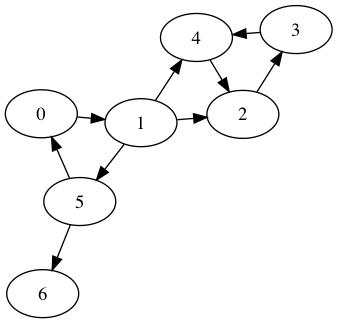
\includegraphics[width=\linewidth]{images/tarjan/0.png}
\caption{Initial graph.} \label{fig:tarjan0}
\end{subfigure}
\hspace*{\fill} % separation between the subfigures
\begin{subfigure}{0.3\textwidth}
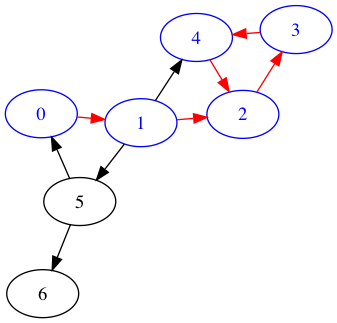
\includegraphics[width=\linewidth]{images/tarjan/1.png}
\caption{The search follows the path $0 \rightarrow 1 \rightarrow 2 \rightarrow 3 
\rightarrow 4 \rightarrow 2$.} \label{fig:tarjan1}
\end{subfigure}
\hspace*{\fill} % separation between the subfigures
\begin{subfigure}{0.3\textwidth}
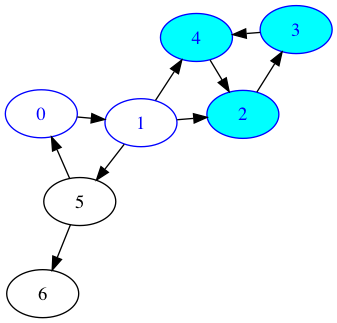
\includegraphics[width=\linewidth]{images/tarjan/2.png}
\caption{Since $lowlink[2] = 2$, nodes 2, 3 and 4 are added into a component.} \label{fig:tarjan2}
\end{subfigure}

\vspace{1cm}

\begin{subfigure}{0.3\textwidth}
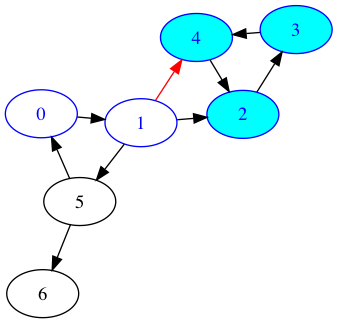
\includegraphics[width=\linewidth]{images/tarjan/3.png}
\caption{The search follows the path $1 \rightarrow 4$, but node $4$ has already been visited.} \label{fig:tarjan3}
\end{subfigure}
\hspace*{\fill} % separation between the subfigures
\begin{subfigure}{0.3\textwidth}
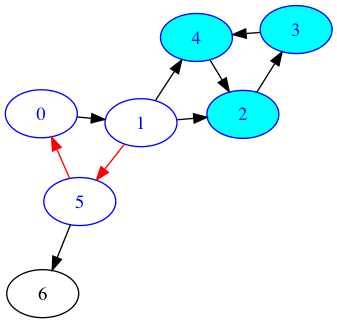
\includegraphics[width=\linewidth]{images/tarjan/4.png}
\caption{The search follows the path $1 \rightarrow 5 \rightarrow 0$.} \label{fig:tarjan6}
\end{subfigure}
\hspace*{\fill} % separation between the subfigures
\begin{subfigure}{0.3\textwidth}
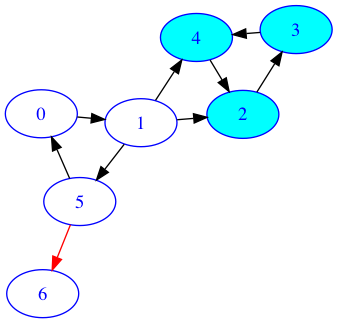
\includegraphics[width=\linewidth]{images/tarjan/5.png}
\caption{The search follows the path $5 \rightarrow 6$.} \label{fig:tarjan5}
\end{subfigure}

\vspace{1cm}

\begin{subfigure}{0.3\textwidth}
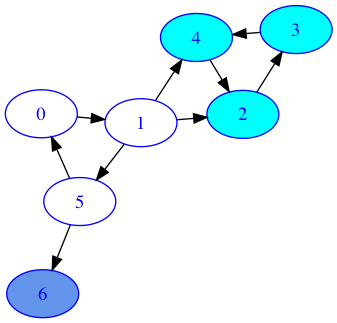
\includegraphics[width=\linewidth]{images/tarjan/6.png}
\caption{Node $6$ does not have outgoing edges and is added to a component.} \label{fig:tarjan6}
\end{subfigure}
\hspace*{2cm} % separation between the subfigures
\begin{subfigure}{0.3\textwidth}
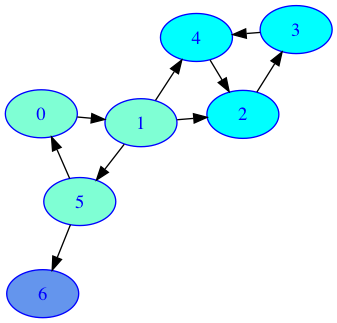
\includegraphics[width=\linewidth]{images/tarjan/7.png}
\caption{The algorithm returns to 0 and, since $lowlink[0] = 0$, adds 0, 1 and 5 to a component.} \label{fig:tarjan7}
\end{subfigure}


\caption{Example of an execution of Tarjan's strongly connected components algorithm.}\label{fig:tarjan}
\end{figure}

\autoref{fig:tarjan} illustrates the execution of Tarjan's algorithm.
The algorithm starts from node 0, with $index[0] = 0$ and $lowlink[0] = 0$.
With a depth-first search, the algorithm traces the path $0 \rightarrow 1 \rightarrow 2 \rightarrow 3 
\rightarrow 4 \rightarrow 2$.
Since node $2$ has already been visited and nodes 4 and 3 have no further outgoing edges, $lowlink[4]$ and $lowlink[3]$ receive the value 2 and the function calls return back to the first visit of node $2$.
At this point, nodes 2, 3 and 4 all have 2 as the smallest reachable index and, therefore, they form a strongly connected component.

Continuing from node 1, the algorithm traces $1 \rightarrow 5 \rightarrow 0$, but stops there since node 0 has already been visited.
Continuing from node 5, the algorithm traces $5 \rightarrow 7$.
Node 7 has no outgoing edges, so it forms a strongly connected component by itself.
Once the function calls return to node 0, a strongly connected component is formed with nodes 0, 1, and 5, since they all have 0 as their $lowlink$ value.

\section{Graph coloring with minimum colors}
\label{section:coloring}
%The algorithm proposed in \citep{mittal2011graph} is an efficient approach to graph coloring, a classic graph theory problem.
Graph coloring is one of the possible heuristics used by TruMan to detect malicious nodes after the generation of the component graph using Tarjan's algorithm.
Out of the tested heuristics, it presents the best results, so it has been chosen as the heuristic for the trust model.

The process of graph coloring consists of giving each node a label (represented by a color) so that no two neighboring nodes share the same color.
This problem has been studied in Computer Science since, at least, 1972 \citep{karp1972reducibility} and has been studied as a classic mathematics problem for even longer \citep{kempe1879geographical}.
It has been proven mathematically that any planar graph can be colored with at most four colors \citep{appel1976every}, but discovering the smallest number of colors necessary to color an arbitrary graph (called the graph's chromatic number) is an NP-hard problem \citep{sanchez1989determining}.

In \citep{mittal2011graph}, the authors present an efficient approach to graph coloring using the minimum possible amount of colors.
Although they do not prove that their algorithm always uses the smallest possible amount of colors, the output is always a correct coloration and the algorithm is nevertheless efficient.
For the purposes of this study, it is not necessary to prove that the coloring algorithm's output uses the minimum possible number of colors.

The complexity of the algorithm is $O(|E'|)$ for a graph $C = (V',E')$.
As a comparison, the DSATUR algorithm for graph coloring has complexity $O(|V|^2)$ \citep{brelaz1979new}.

Algorithm \autoref{algorithm:coloring} shows the general structure of the graph coloring algorithm  \citep{mittal2011graph}.

\begin{algorithm}
\caption{Graph coloring with minimum colors}\label{algorithm:coloring}
\begin{algorithmic}[1]

\Function{Coloring}{graph $G$}

\State \textbf{color} all nodes of $G$ \textbf{with} 0
\State $d \rightarrow 0$
\For{$e=(u,v)$ \textbf{in} edges of $G$}
	\If{$u$ and $v$ have the same color}
		\If{$color[v] = d$}
			\State $d \rightarrow d+1$
		\EndIf
		\State $color[v] \rightarrow d$
	\EndIf
\EndFor


\EndFunction
\end{algorithmic}
\end{algorithm}


\begin{figure}
\centering

\begin{subfigure}{0.20\textwidth}
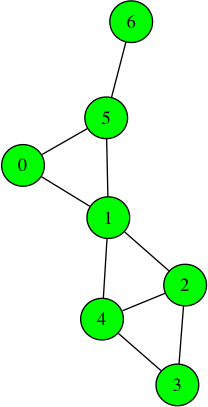
\includegraphics[width=\linewidth]{images/coloring/0.png}
\caption{Initial graph with all nodes labeled 1. $d=1$ (green).\\} \label{fig:coloring0}
\end{subfigure}
\hspace*{\fill} % separation between the subfigures
\begin{subfigure}{0.20\textwidth}
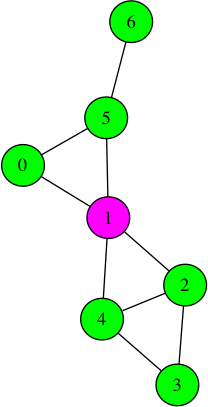
\includegraphics[width=\linewidth]{images/coloring/1.png}
\caption{Edge $(0,1)$ is checked and node $1$ gets a new color. $d=2$ (magenta).} \label{fig:coloring1}
\end{subfigure}
\hspace*{\fill} % separation between the subfigures
\begin{subfigure}{0.20\textwidth}
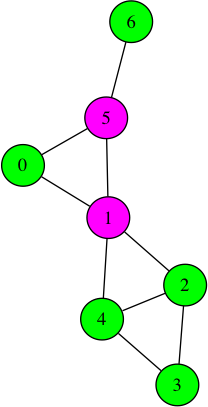
\includegraphics[width=\linewidth]{images/coloring/2.png}
\caption{Edge $(0,5)$ is checked and node $5$ gets the current value of $d$.} \label{fig:coloring2}
\end{subfigure}
\hspace*{\fill} % separation between the subfigures
\begin{subfigure}{0.20\textwidth}
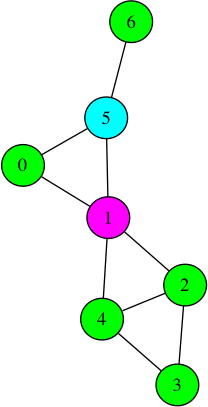
\includegraphics[width=\linewidth]{images/coloring/3.png}
\caption{Edge $(1,5)$ is checked and node $5$ gets a new color. $d=3$ (cyan).} \label{fig:coloring3}
\end{subfigure}

\vspace{2cm}

\begin{subfigure}{0.20\textwidth}
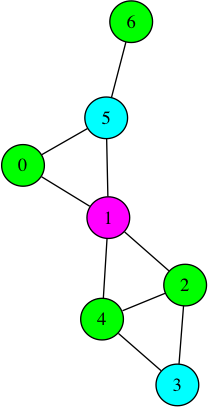
\includegraphics[width=\linewidth]{images/coloring/4.png}
\caption{Edge $(2,3)$ is checked and node $3$ gets the current value of $d$.} \label{fig:coloring5}
\end{subfigure}
\hspace*{2cm} % separation between the subfigures
\begin{subfigure}{0.20\textwidth}
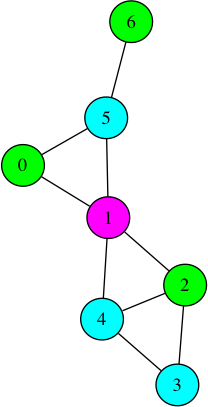
\includegraphics[width=\linewidth]{images/coloring/5.png}
\caption{Edge $(2,4)$ is checked and node $4$ gets the current value of $d$.} \label{fig:coloring6}
\end{subfigure}
\hspace*{2cm} % separation between the subfigures
\begin{subfigure}{0.20\textwidth}
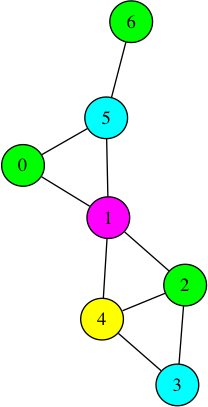
\includegraphics[width=\linewidth]{images/coloring/6.png}
\caption{Edge $(3,4)$ is checked and node $4$ gets a new color. $d=4$ (yellow).} \label{fig:coloring6}
\end{subfigure}

\caption{Example of an execution of the graph coloring with minimum colors algorithm.}\label{fig:coloring}
\end{figure}

A limitation of this algorithm is that the edges must be sorted according to node indexes.
It doesn't matter which nodes get assigned which indexes, but once they are assigned those numbers, the algorithm must follow the edges in numerical order.
This is demonstrated in \citep{vernize2013dissertation}.

Figure \autoref{fig:coloring} illustrates the execution of the graph coloring algorithm.
It is notable how few iterations the algorithm takes to fully color the graph.
However, the fact that the result does not use the minimum amount of colors.
By coloring node 4 as cyan and node 3 as magenta, the sample graph could have been colored with only three colors.
However, as described above, this is not a substantial problem for the purposes of this study.

\section{Malicious Node Identification Algorithm}

The basis of TruMan is the Malicious Node Identification Algorithm (MaNI) proposed in \citep{vernize2015malicious}, which suggests the use of strongly connected components and graph coloring for malicious node detection.
This article presents a malicious node identification scheme based on strongly connected components and graph coloring.
The model is proposed for complex networks in general, but is not suited for VANETs because it is designed only for static networks.
Furthermore, the algorithm is executed by a global observer which has information about the complete network.

The input graph $T = (V,E)$ is a static, connected, and directed graph containing all trust relationships in the network.
Such relationships are binary, so there are no varying degrees of trust: either one node trusts another completely (edge value is $1$), or it distrusts the other completely (edge value is $0$).
The relationships are also directed, meaning that if the value of $A\rightarrow B$ is $1$, $B\rightarrow A$ is not necessarily $1$.

The process for identifying malicious nodes within $T$ is as follows:

First, $T$ is separated into strongly connected components using Tarjan's algorithm \citep{tarjan1972depth}, which is described in detail in \autoref{section:tarjan}.
In each of these components, all nodes are connected by edges of value $1$.
In other words, within a single component, all nodes trust one another; nodes connected by edges of value $0$ are separated into different components.
Each of these components becomes a node of a component graph $C = (V', E')$.

The creation of the graph $C$ simplifies the remaining computation.
Since each node of $C$ is a vertex $v' \in V'$ and each vertex $v'$ is a component of $T$ in which all nodes trust each other, for the purposes of identifying malicious nodes, all nodes within each of those components can be treated as one.
They can either be benign nodes which legitimately trust one another, or malicious nodes colluding with each other.
After the formation of $C$, one or more heuristics can be used to classify the nodes as benign or malicious.

The article describes the coloring heuristic, which uses a graph coloring algorithm, either DSATUR \citep{brelaz1979new} or the algorithm proposed in \citep{mittal2011graph}.
Graph coloring is a classic problem of graph theory, in which the objective is to assign each node in a graph a color so that no two neighboring nodes share the same color.
After running either algorithms with graph $C$, the color whose nodes in $C$ represent the most nodes in $T$ is classified as correct, and all others are classified as malicious.
Once this information in $C$ is brought back to graph $T$, it is trivial to label the nodes in $T$ as either benign or malicious based on their components' classifications.

In the experiments shown in \citep{vernize2013dissertation}, the coloring heuristic shows the most promising results, identifying a high ratio of the malicious nodes in the network.
Other heuristics were experimented with, but were either less effective in detecting malicious nodes, or provided too many false positives.
Therefore, for the purposes of this research, only the coloring heuristic is considered.

Two types of experiments were made in each network: first, all malicious nodes inverted the edge weights leading to their neighbors; second, malicious nodes randomly inverted or not the weights.
In the first scenario, the results show excellent precision in most networks, detecting nearly every malicious node.
Experimenting with the second scenario, the results are less precise, however still promising: with up to 20\% of malicious nodes in the network, the error rate is under 7\%, while with the worst case, 50\% of the network being malicious, the error rate is approximately 15\%.

The authors suggest running the algorithm repeatedly after removing the malicious nodes from the network.
By doing this, nearly all malicious nodes are detected by it even when randomly changing edge weights.

%\begin{algorithm}
%\caption{MaNI algorithm}\label{algorithm:mani}
%\begin{algorithmic}[1]
%
%\Function{MaNI}{graph $T$}
%
%\State $C \gets$ \textbf{Tarjan}$(T[0])$
%\State $colors \gets$ \textbf{Coloring}$(C)$
%\State \textbf{color} nodes of $T$ \textbf{according to} $colors$
%\State \textbf{count} 
%
%\EndFunction
%\end{algorithmic}
%\end{algorithm}

\begin{figure}
\centering

\begin{subfigure}{0.25\textwidth}
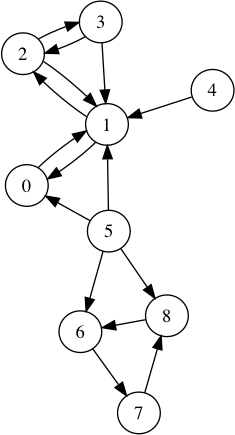
\includegraphics[width=\linewidth]{images/mani/0-trust.png}
\caption{Initial graph $T$.} \label{fig:mani0}
\end{subfigure}
\hspace*{2cm} % separation between the subfigures
\begin{subfigure}{0.25\textwidth}
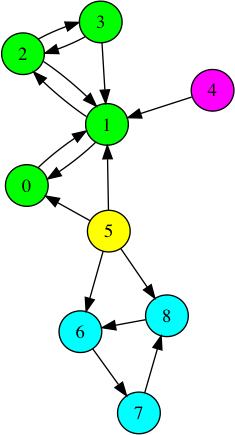
\includegraphics[width=\linewidth]{images/mani/1-tarjan.png}
\caption{Tarjan's algorithm is used to identify the strongly connected components.} \label{fig:mani1}
\end{subfigure}


\vspace{1cm} % separation between the subfigures

\begin{subfigure}{0.3\textwidth}
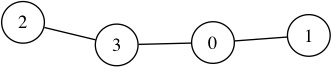
\includegraphics[width=\linewidth]{images/mani/2-components.png}
\caption{The graph $C$ is formed from the components of $T$.} \label{fig:mani2}
\end{subfigure}
\hspace*{2cm} % separation between the subfigures
\begin{subfigure}{0.3\textwidth}
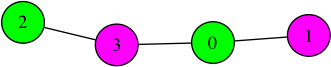
\includegraphics[width=\linewidth]{images/mani/3-colored-components.png}
\caption{The coloring algorithm is used to label the nodes of $C$.} \label{fig:mani3}
\end{subfigure}

\vspace{1cm} % separation between the subfigures

\begin{subfigure}{0.25\textwidth}
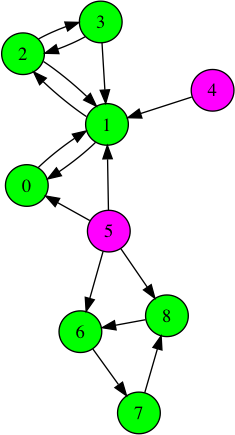
\includegraphics[width=\linewidth]{images/mani/4-result.png}
\caption{The colors from $C$ are used to label nodes in $T$ as correct or malicious.} \label{fig:mani4}
\end{subfigure}


\caption{Example of an execution of the MaNI algorithm.}\label{fig:mani}
\end{figure}


\autoref{fig:mani} illustrates the execution of the MaNI algorithm.
With the starting graph $T$, whose edges represent the trust relationships between nodes, Tarjan's strongly connected component algorithm is executed.
\autoref{fig:mani1} shows nodes colored according to their placement in a strongly connected component.
The strongly connected components form a graph $C$ according to edges present in $T$.
In \autoref{fig:mani2}, component $0$ is the one containing node $5$; component $1$ contains nodes $6$, $7$ and $8$; component $2$ contains nodes $0$, $1$, $2$ and $3$; and component $3$ contains node $4$.
The graph coloring with minimum colors algorithm is executed on $C$, producing the coloration shown in \autoref{fig:mani3}.
Finally, each node in $T$ is colored according to which color its component received in $C$.
The color with the most nodes is deemed benign, while the others are considered malicious. 


%$G = (V,E)$: undirected topology graph, in which $V$ are the vertices and $E$ are the edges.
%
%$T = (V,O)$: directed trust graph, in which $O$ are the nodes' opinions about each other.
%
%$G_t,T_t$: snapshots of $G$ and $T$ in a timestamp $t$.
%
%$G_i,T_i$: local knowledge of $G$ and $T$ of a node $i$.
%
%$C = (V',O')$: component graph of $T$.


\section{The TruMan algorithm}
\label{section:algorithm}

TruMan is based on the MaNI algorithm \citep{vernize2015malicious}, which suggested the use of Tarjan's algorithm and the graph coloring algorithm.
However, MaNI was developed for static networks such as social networks, and is executed by an external supervising agent (i.e. outside of the network), making it unsuitable for a vehicular network.

In order to work with dynamic networks, the TruMan algorithm runs iterations at predetermined intervals.
%As nodes acquire more information, their model of the network will change.
Furthermore, the algorithm runs in a decentralized fashion, meaning each node in the network runs its own instance of the algorithm.
Each node starts knowing information only about itself and maintains its own abstraction of the network surrounding it.
Every node $u$ stores a representation of the network in the form of a static, connected and directed trust graph $T = (V, E)$, in which $V$ is the set of nodes node $u$ is aware of and $E$ is the set of trust relationships (opinions) $u$ knows between members of $V$.
Since each node has its own network representation and it changes over time, there is a $T^u_i = (V^u_i, E^u_i)$ for every node $u$ and iteration $i$.

At first, the node collects and organizes information.
A prerequisite of this step is a test that correctly classifies a neighboring node as benign or malicious.
There are several ways to perform such a test, but a study between these methods is beyond the scope of this paper.
Every time a neighboring node $v$ is tested as benign, the value of $u \rightarrow v$ increases and the trust graph $T^v_{i-1}$ is merged into $u$'s trust graph.
After this, a new $T^u_i$ is formed, which is used for the remaining steps.

After the collection of data, $T^u_i$ is separated into strongly connected components using Tarjan's algorithm \citep{tarjan1972depth}.
For each node in a component, there is a path formed by edges of weight higher than the threshold $h$ to each other node in the same component.
In other words, within a single component, all nodes trust one another directly or indirectly; nodes that do not satisfy this condition are separated into different components.
Each of these components becomes a node of a component graph $C^u_i = (V'^u_i, E'^u_i)$.

The creation of $C^u_i$ simplifies the remaining computation.
Since each vertex $v' \in V'^u_i$ is a component of $T^u_i$ in which all nodes trust each other, for the purposes of identifying malicious nodes, all nodes within each of those components can be treated as the same.
They can either be benign nodes which legitimately trust one another, or malicious nodes colluding with each other.
After the formation of $C^u_i$, a heuristic is used to classify the nodes as benign or malicious.

The coloring heuristic is used to classify nodes, which uses the algorithm described in \autoref{section:coloring} \citep{mittal2011graph}, although other heuristics may be considered.
After running the graph coloring algorithm with graph $C^u_i$ as input, the color whose nodes in $C^u_i$ represent the most nodes in $T^u_i$ is classified as correct, and all others are classified as malicious.
Once this information from $C^u_i$ is brought back to graph $T^u_i$, it is trivial to label the nodes in $T^u_i$ as either benign or malicious based on the classifications of their components.

The complexity of the whole algorithm can be calculated by adding the most costly operations involved.
As discussed above, Tarjan's algorithm has a complexity of $O(|V|+|E|)$ (for the trust graph $T$), while the graph coloring algorithm has a complexity of $O(|E'|)$ (for the component graph $C$).
The most costly part of the algorithm is the graph merge operation that happens between trusted nodes.
The complexity of the graph merge algorithm is $O(|E|)$ for each neighbor a node has in an iteration; this number is at most $|V|$.
The total complexity of TruMan is, therefore, $O(|V|+|E|)+O(|E'|)+O(|V|\times |E|)$.
Since $|E'| \leq |E|$ and $|V|+|E| \leq |V|\times |E|$, the complexity can be simplified to $O(|V| \times |E|)$.

In summary, every node $u$ runs the following steps in each iteration to detect malicious nodes in the network:

\begin{enumerate}
	\item Node $u$ checks which are its neighbors (nodes within its communication range).
		  New discovered nodes and new formed edges are added to $T^u_i$.
		  Edges are created with weight 0.5.
	\item Node $u$ tests all its neighbors to discover which ones can be directly trusted or not.
		  New trust values are computed for the edges using the average between the previous value and either 1 (if the neighbor is trustworthy) or 0 (otherwise).
	\item If a neighbor $v$ is trustworthy, $u$ merges $T^v_{i-1}$ into $T^u_i$.
	\item Tarjan's algorithm is executed to identify the strongly connected components of $T^u_i$, resulting in a component graph $C^u_i$.
	\item The graph coloring algorithm is executed on $C^u_i$ and nodes are classified as benign or malicious.
\end{enumerate}


%The MaNI algorithm works well and is efficient for static graphs.
%However, some important modifications had to be made to accommodate dynamic graphs.
%The main changes made are described below.
%
%\subsection{Graph knowledge and graph building}
%First of all, there is an important change to the graph knowledge used to run the algorithm.
%The complete trust graph is a parameter to the MaNI algorithm, which executes with complete knowledge of the graph.
%
%Given the complete topology graph $G = (V, E)$, each node $u \in V$ has its own vision of the network and $u$ has to build a graph, $G_u$, to represent its surrounding network.
%In each iteration of the algorithm, $u$ receives information from its neighbors about their own graphs.
%For every neighbor $v \in V$, $G_u$ must me merged with $G_v$.
%In sufficient iterations, $G_u$ forms a complete or nearly complete vision of the network.
%
%Alongside $G$, there is the trust graph $T = (V, O)$ which stores trust relationships between pairs of nodes in the form of directed edges.
%Again, each node $u$ has its own $T_u$, which contains the trust information node $u$ knows about.
%When a node $u$ asks for network information from node $v$, it also merges $T_u$ with $T_v$, but only if $u$ trusts $v$.
%If $u$ deems $v$ malicious, any information originating from $v$ cannot be considered valid.
%
%[Illustrate graph building here]
%
%Furthermore, this implies that the malicious node detection algorithm runs using incomplete graph knowledge.
%This is expected and generally unavoidable in vehicular networks, which have high mobility and can be extremely large.
%
%
%
%-\\
%----------\\
%This paragraph is probably pertinent to delimiting the size of graphs:\\
%The authors of \citep{patwardhan2006data} provide important observations regarding the collection of data from local conditions.
%Most crucially, they mention how the quality of information is higher when the origin of such information is close to the destination node.
%That is, data collected by the node's own sensors have the highest quality, which diminishes as information starts to come from neighbors, neighbors of neighbors and so forth.
%They adopt a broadcast model in which RSUs send data about its surroundings and OBUs capture the information.
%The trust model proposed here might use a similar broadcast model, although adapted so all nodes are vehicles (OBUs).\\
%----------\\

%The original work's scope does not include the generation of the trust graph, as it is a parameter to the algorithm.
%In dynamic graphs, trust relationships change over time, so how those changes affect the proposed trust model have to be considered.
%This includes not only the full figure of the graph, but also each node's views on its neighbors.
%
%\subsection{Strongly connected components}
%Strongly connected components, or components in which all nodes have positive trust relationships with each other, are somewhat different in dynamic graphs.
%As nodes enter, leave, or change locations in the network, the components change accordingly.
%Therefore, our algorithm will have to work using ``snapshots'' of the graph, meaning each measurement will be valid for a specific timestamp.
%Since the graph changes with time, for every timestamp $t$, there is a corresponding topology graph $G_t=(V_t, E_t)$, which includes the available vertices and edges in that moment in time, and a trust graph $T_t=(V_t, O_t)$, with the nodes' opinions at that moment.
%
%In a later step, it might be useful to consider how specific nodes may change over several snapshots.
%Specifically, the suggestion of running the algorithm in iterations, by removing the malicious nodes in each step, may be applied with the peculiarities of a dynamic network.
%
%\subsection{Graph knowledge}
%In the original paper, the malicious nodes are identified by a central entity with access to all nodes' trust values.
%Not only does our work plan to decentralize this procedure, having complete knowledge of the graph is unfeasible in large-scale dynamic networks such as VANETs.
%Therefore, our algorithm needs to work using only a partial understanding of the network.
%For this to be viable, each node might have to gather information not only from its views on its neighbors, but also from its neighbors' views.
%
%The authors of \citep{patwardhan2006data} provide important observations regarding the collection of data from local conditions.
%Most crucially, they mention how the quality of information is higher when the origin of such information is close to the destination node.
%That is, data collected by the node's own sensors have the highest quality, which diminishes as information starts to come from neighbors, neighbors of neighbors and so forth.
%They adopt a broadcast model in which RSUs send data about its surroundings and OBUs capture the information.
%The trust model proposed here might use a similar broadcast model, although adapted so all nodes are vehicles (OBUs).
%
%Thus, each node has its own model of the network topology, $G_i$, and generates a trust graph $T_i=(V_i, O_i)$, in which $i$ is the node's identifier.
%Combined with the necessity of timestamps explained above, this results in a graph $T_{it}=(V_{it}, O_{it})$ for each node and each timestamp, which is the input of the new algorithm.
%Accordingly, there are also component graphs $C_{it}=(V'_{it}, O'_{it})$, generated on each instance of the algorithm.
%
%During the early stages of development, it will be considered that vertices cannot enter or leave the network and, therefore, only the layout of the edges changes.
%This is sufficient to experiment with the algorithm's performance with the added complexity of a dynamic network.
%
%
%\subsection{Binary trust}
%A model using binary trust is one in which trust values can only be 0 or 1.
%If node $A$ positively trusts node $B$, the value of the edge $A\rightarrow B$ is 1.
%If it does not trust $B$, or is unsure, the value is 0.
%Such a scheme makes sense in a static graph but, in a dynamic one, it is interesting to have a range of possible trust values.
%
%Since nodes interact with each other occasionally and might learn information from other nodes, a range of $[0,1]$ is useful to express how one trust value can change over time.
%As one node learns more about another, the value can grow or diminish and, once it goes above or below a certain threshold, the neighboring node can be deemed trustworthy or not.
%The rate in which trust increases or decreases must be experimented with; it could be useful to have trust decrease faster than it increases, but that might also cause false positives in the case of occasional mistakes.
%
%\subsection{Datasets}
%The datasets used for experimentation must be changed accordingly.
%Instead of using data gathered from social networks, which are static, dynamic network datasets must be used, such as traffic information for cities.
%
%At first, the objective is to test using the Working Day Movement Model, setting parameters that contribute to the validation of the algorithm.
%When the simulation begins, a set number of nodes are malicious and, therefore, other nodes will have low trust in them after interacting.
%In time, benign and malicious nodes can change their behavior and, accordingly, their trustworthiness will be updated.
%
%It might still be useful to simulate using real-world movement traces.
%An example of such dataset is the Zurich Trace \citep{zurichtrace}, which describes the vehicular traces in the city of Zurich, Switzerland.
%The chosen dataset doesn't necessarily need to be created for VANETs, since with vehicular traces it is possible to assume all or a percentage of the traced vehicles are smart and can be nodes of a hypothetical VANET.
%The mobility of the nodes is the most important aspect of the dataset.